\subsection{Code comparison: Tendril case} \labsec{tendril case}

\begin{figure*}
    \centering
    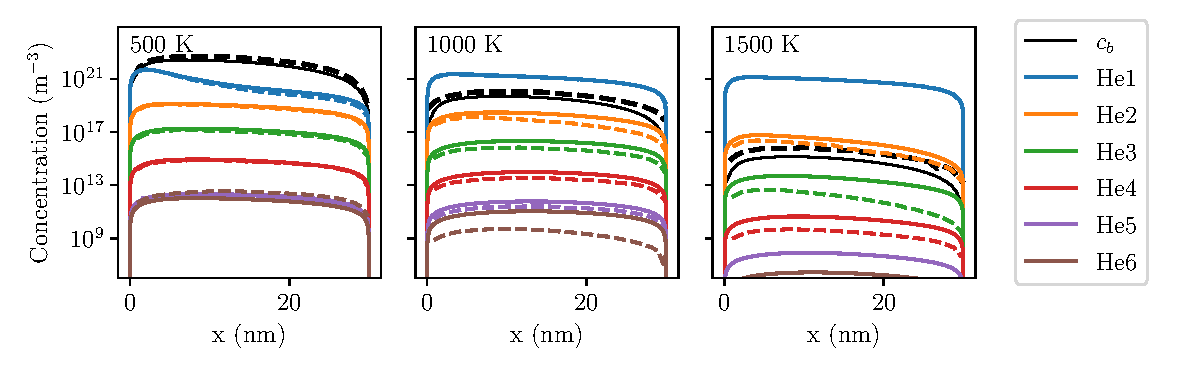
\includegraphics[width=\linewidth]{Figures/Chapter4/profiles_tendrils.pdf}
    \caption{He clusters concentration profiles in the \gls{tendril} at \SI{500}{K}, \SI{1000}{K} and \SI{1500}{K} under \SI{100}{eV} He exposure at \SI{1e22}{m^{-2}.s^{-1}} at a fluence of \SI{5e25}{m^{-2}}. Comparison between the current implementation (solid) and Faney's results \cite{faney_spatially_2015} (dashed).}
    \labfig{tendril profiles}
\end{figure*}

The current implementation was compared to literature results\cite{faney_spatially_2015}.
Helium exposure in a \gls{tendril} was simulated in 1D.
The helium flux is \SI{1e22}{m^{-2}.s^{-1}} and the fluence was \SI{5e25}{m^{-2}}.

The domain size is \SI{30}{nm} and the volumetric source term is described as follows:
\begin{equation}
    \Gamma(x) = \varphi_\mathrm{imp} \; f(x) 
\end{equation}
where $\varphi_\mathrm{imp} = \SI{1e22}{m^{-2} s^{-1}}$ is the implanted He flux and $f(x)$ is a Gaussian distribution with a mean value $\mu = R_p = \SI{1.5}{nm}$ and a standard deviation $\sigma = \SI{1}{nm}$ which corresponds to a \SI{100}{eV} He implantation based on \gls{srim} computations \sidecite{ziegler_srim_2010}.

Mobile He clusters concentrations were set to zero at the \gls{tendril}'s surfaces ($x=\SI{0}{nm}$ and $x=\SI{30}{nm}$).

Concentration profiles computed by the current implementation showed good agreement with the ones obtained by Faney et al.\ \cite{faney_spatially_2015} (see \reffig{tendril profiles}).
The discrepancies are likely due to a difference in the set of dissociation energies that have been used as these energies have an impact on the concentration profiles (see \reffig{parametric study dissociation energies}).
Indeed, at low temperature, where dissociation is not activated, the discrepancies were rather small whereas at high temperature, differences increased because dissociation became more dominant.

\begin{figure*}
    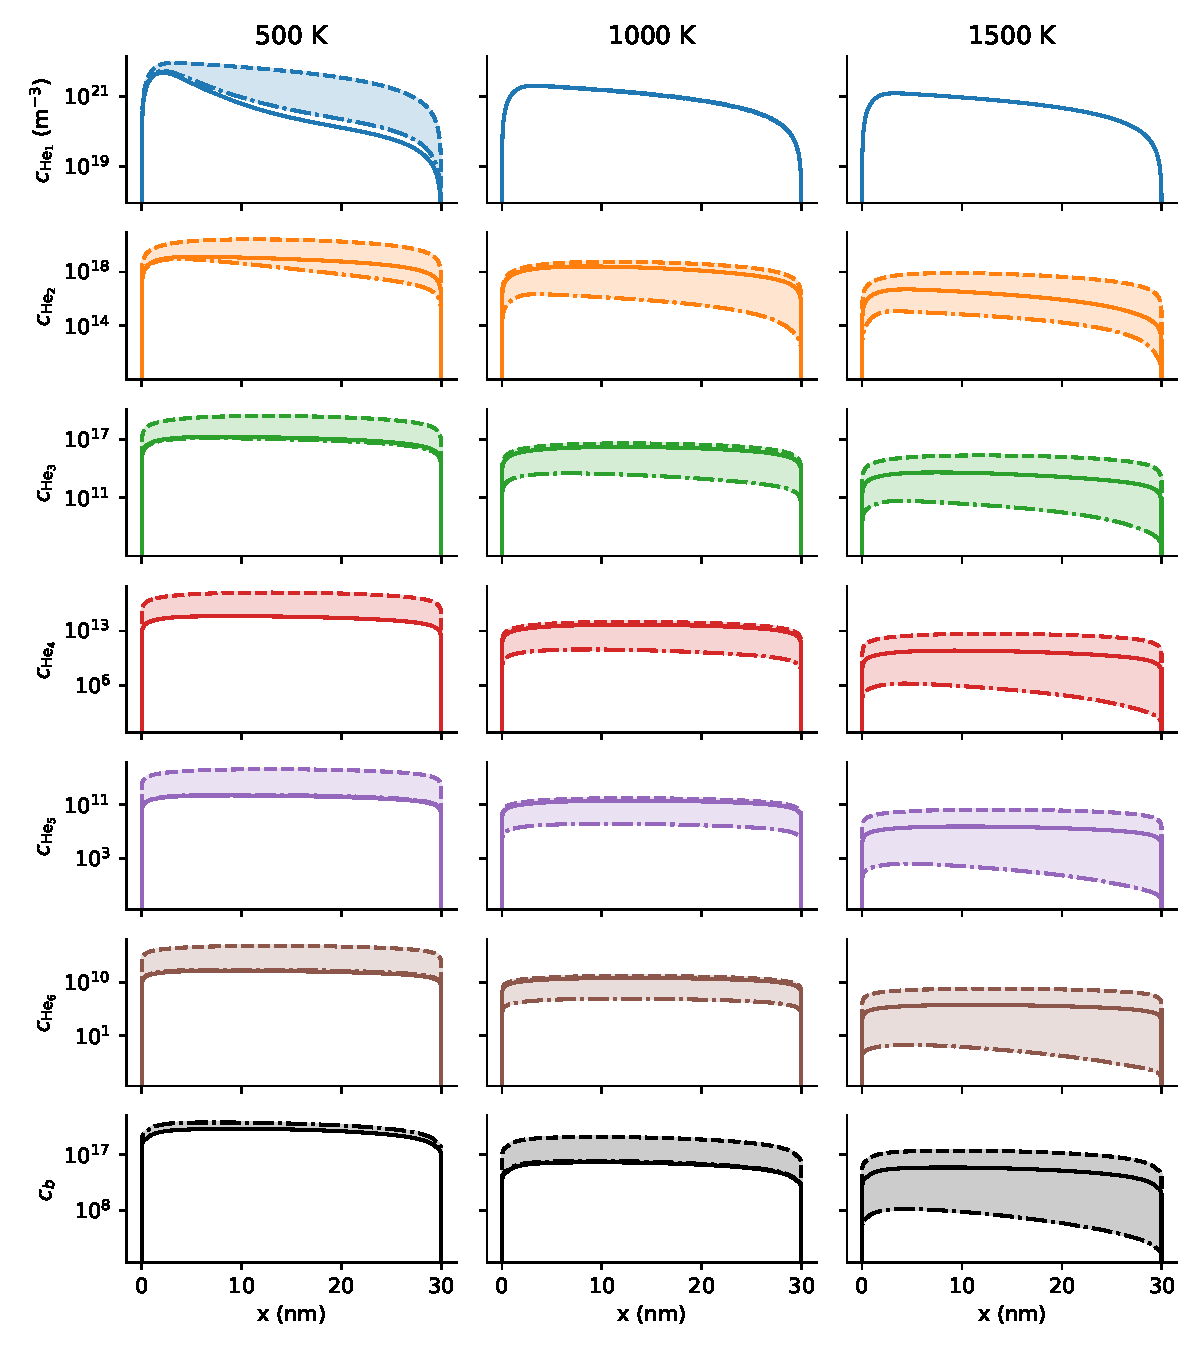
\includegraphics[width=\linewidth]{Figures/Chapter5/parametric_study_dissociation_energies.pdf}
    \caption{Helium clusters concentration profiles on the tendril case with dissociation energies varying from -\SI{0.5}{eV} (dash-point) to +\SI{0.5}{eV} (dash).}
    \labfig{parametric study dissociation energies}
\end{figure*}

% When $c_b$ is small compared to $c_{\mathrm{He}_1}$, the equilibrium of $\mathrm{He}_1$ is independent of these dissociation energies and the profiles for $\mathrm{He}_1$ are identical.

Moreover, increasing the temperature tended to inhibit bubble formation in the \gls{tendril}.
This was explained by a greater increase in the dissociation rate and in losses at surfaces than the increase in the clustering rate.
This observation is in agreement with \gls{md} results simulating He implantation in \glspl{tendril} \sidecite{wei_better_2020, wei_understanding_2019}.
The current implementation and the additional assumptions that were made are therefore valid.

\subsection{Comparison with experiments}

\begin{figure} [h]
    \centering
    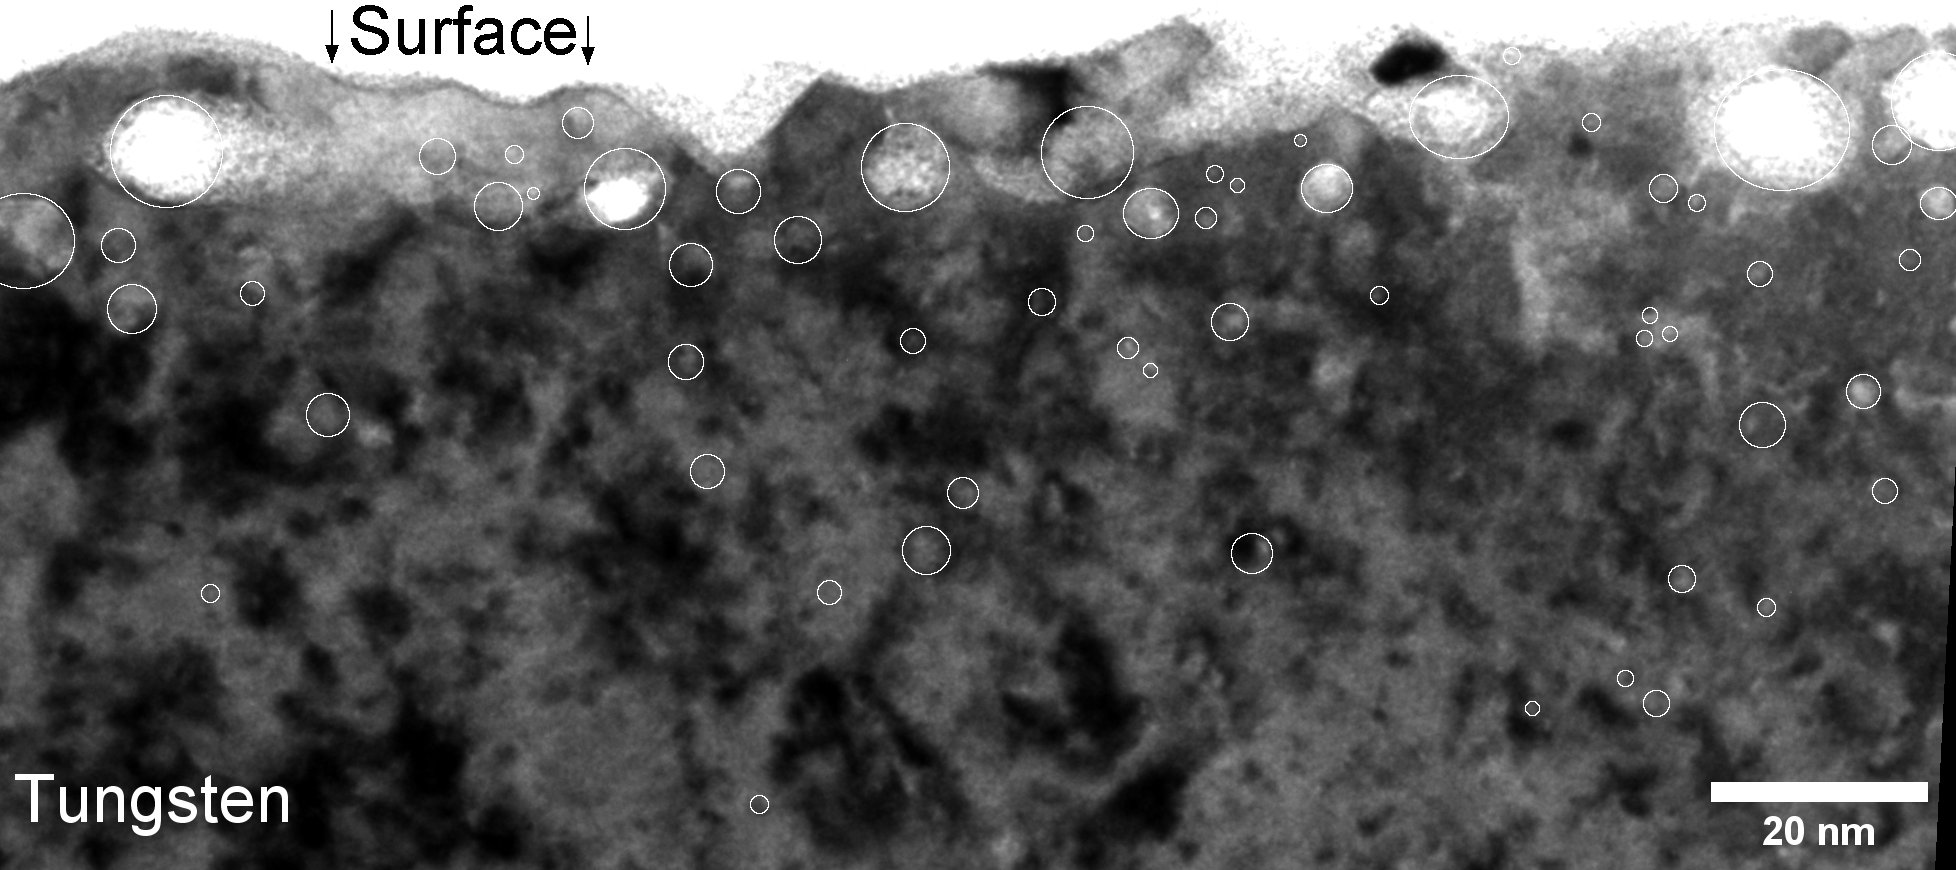
\includegraphics[width=\linewidth]{Figures/Chapter4/bubbles_tem.jpg}
    \caption{\gls{tem} images of W after exposure to \SI{75}{eV} He at \SI{2.3e22}{m^{-2}.s^{-1}} and \SI{1053}{K} for \SI{13}{s} showing bubbles that have burst, large size bubbles at the near surface and small size bubbles in the bulk.}
    \labfig{tem images}
\end{figure}

\begin{figure} [h!]
    \centering
    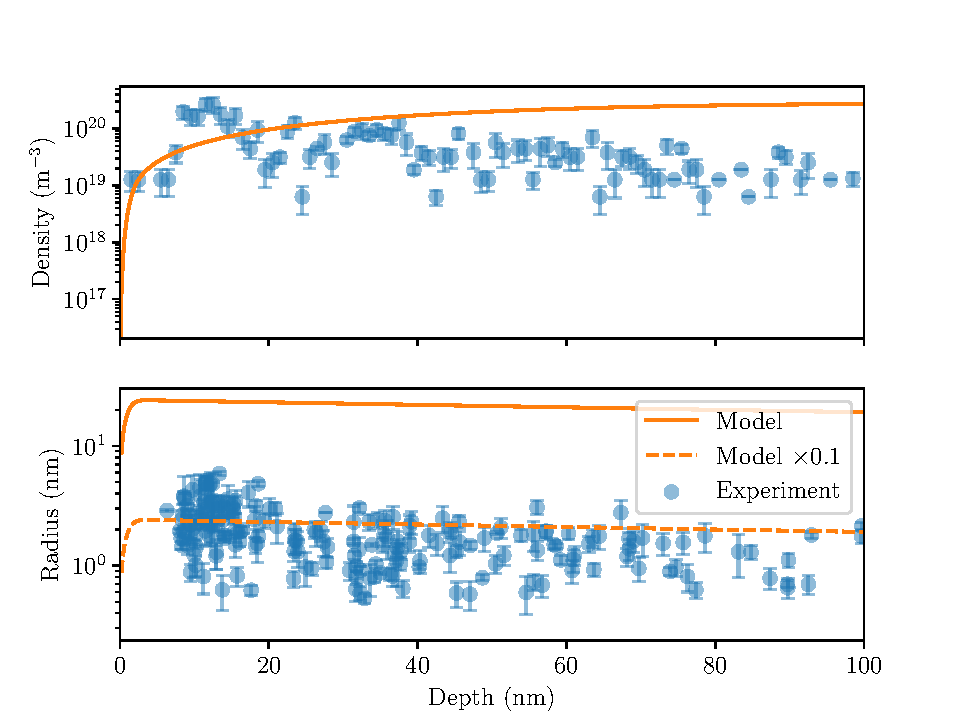
\includegraphics[width=\linewidth]{Figures/Chapter4/comparison_model_exp.pdf}
    \caption{Comparison of experimental results with simulations for W implanted with \SI{75}{eV} He at \SI{2.3e22}{m^{-2}.s^{-1}} and \SI{1053}{K} for \SI{13}{s}. Error bars correspond to the lowest and highest radius in the \gls{tem} image.}
    \labfig{exp model comparison}
\end{figure}

% He implantation experiments were performed on W and TEM (Transmission Electron Microscopy) images were produced (see \reffig{tem images}).
% W was irradiated with \SI{75}{eV} He at \SI{2.3e22}{m^{-2}.s^{-1}} and \SI{1053}{K} for \SI{13}{s}.
% Comparison of under- and over-focused TEM images allowed identification of the bubbles.
% say something about the imaging technique or the lamella...

He implantation experiments were performed on W in the linear plasma device PSI--2 \sidecite{kreter_linear_2015}.
W was irradiated with \SI{75}{eV} He at \SI{2.3e22}{m^{-2}.s^{-1}} and \SI{1053}{K} for \SI{13}{s}.
A thin lamella for cross-sectional observations was prepared using the \gls{fib} technique with a Dual Beam FIB (FEI Helios 600 NanoLab).
Prior to \gls{fib} cutting, the surface of the sample was coated with a SiO layer for better contrast and then with a protective platinum layer to avoid damaging the surface during the lamella preparation.
Cross-sectional observations of the He-implanted W were performed using \gls{tem} in a TEM FEI Titan 80-300 apparatus.

A typical \gls{tem} image of the lamella is presented in \reffig{tem images}.
Comparison of under- and over-focused \gls{tem} images allowed identification of the bubbles.
Bubbles were observed up to \SI{100}{nm} with larger bubbles closer to the surface and smaller bubbles deeper in the bulk.
Open bubbles and holes at the surface were also observed suggesting bursting events occurred.
This is in accordance with what was observed in the simulations (see \reffig{profiles rb half slab}).

A procedure was developed to automate the bubble detection on \gls{tem} images using the ImageJ software \sidecite{schindelin_fiji_2012}.
The area of bubbles were computed as well as their diameter assuming a spherical shape for the bubbles.
Bubble density and size as a function of depth was therefore computed using 12 pairs of under- and over-focused \gls{tem} images.
The bubble density was found to range from \SI{7e19}{m^{-3}} to \SI{2e20}{m^{-3}} and the bubble radius ranged between \SI{1}{nm} and \SI{10}{nm} (see \reffig{exp model comparison}).
Although the resolution of the \gls{tem} is below \SI{1}{nm}, the number of bubbles with radius below \SI{2}{nm} is underestimated due to the limited contrast.

This experiment was simulated using the same exposure conditions.
The simulated bubbles density $c_b$ was found to be in accordance with the one measured experimentally.
Some discrepancies were found at the near surface.

The bubble radius $\langle r_b \rangle$ is however overestimated by an order of magnitude compared to experimental measurements.
This could imply that the current model linking the He content to the bubble radius is overestimated and that a more accurate one is needed.
Bursting in over-pressurised bubbles close to the surface would also reduce the bubble size. 
Finally, it would be worth investigating this further to determine the impact of initial defects.
